\section{Inductors and Capacitors}

\subsection{Inductors in Series and PArallel}
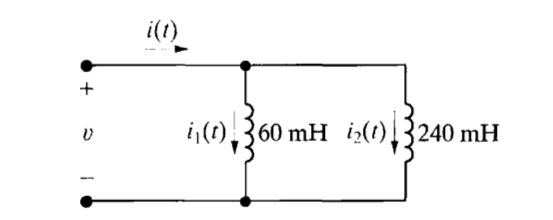
\includegraphics[scale=0.5]{img/c6/p1} \\
The initial value of $i_1$ and $i_2$ in the circuit shown are +3 A and -5 A respectively. The
voltage at the terminals of the parallel inductors for $t \geq 0$ is $-30e^{-5t}$ mV. 

\begin{enumerate}
	\item If the parallel inductors are replaced by a single inductor, what is the inductance?
	\item What i the initial current and its reference direction in the equivalent inductor?
	\item Use the equivalent inductor to find $i(t)$. 
	\item Find $i_1(t)$ and $i_2(t)$. Verify the solutions for $i_1(t)$, $i_2(t)$, and $i(t)$ 
	satisfy Kirchhoff's current law. 
\end{enumerate}

1) First we find the equivalent inductance of the two parallel inductors:

\begin{align*}
	L_{eq} &= \frac{L_1 * L_2}{L_1 + L_2} \\
	L_{eq} &= \frac{60*240}{60+240} \\
	L_{eq} &= 48 mH \\
\end{align*}

2) Next we can find the inital current of the combined inductor by adding
the values of the current through the two individual inductors. \\
\begin{align*}
	i(0^{+}) &= i_{L1} + i_{L2} \\
		 &= 3 + (-5) \\
		 &= -2 A \\
\end{align*}

3) Now we can use the equivalent inductor to find $i(t)$. Remember that the
voltage when t is greater than 0 is given in the problem statement. Also 
notice we just found the current when t = 0.   \\

\begin{align*}
	L_{eq} &= \frac{1}{0.06} + \frac{1}{0.240} \\
	L_{eq} &= \frac{125}{6} \\
	i &= \frac{1}{L_{eq}}\int_{t_0}^{t} v dt + i(t_0) \\
	i &= \left( \frac{125}{6}\right)\int_{0^{+}}{t} (-0.03e^{-5x})dx - 2 \\
	i &= 0.125e^{-5t} - 2.125 A \\
\end{align*}

4) Now we can solve for $i_1(t)$ and $i_2(t)$ as follows: \\
\begin{align*}
	i_1 &= L_{eq} * \left( \frac{L_1}{L1+L2} \right) \int_{t_0}^{t} v dt + i (t_0) \\
	i_1 &= \frac{125}{6} * \left(\frac{0.06}{0.06 + 0.24}\right) \int_{0^{+}}^{t} (-0.03e^{-5x})dx + 3 \\
	i_1 &= 0.1e^{-5t} + 2.9 A \\ 
	i_2 &= \frac{25}{6} \int_{0^{+}}^{t} (-0.03e^{-5x})dx - 5 \\
	i_2 &= 0.025e^{-5t} - 5.025 A \\
	i_1 + i_2 &= i \\
\end{align*}


\subsection{Capacitors in series and parallel}
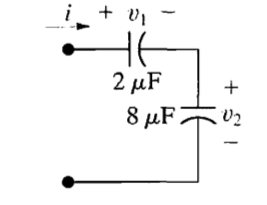
\includegraphics[scale=0.5]{img/c6/p2} \\
The current at the terminals of the two capacitors shown is $240e^{-10t} \mu A$ for $t \geq 0$. The
initial values of $v_1$ and $v_2$ are -10V and -5V respectively. Calculate the total energy trapped
in the capacitors as $t$ approaches $\infty$. 

Using the hint we can see that we should not try to combine the two capacitors and instead should solve for each voltage individually. 
\begin{align*}
	v &= \frac{1}{C}\int_{t_0}^{t} i tx + v(0) \\
	v_1 &= \frac{1}{2 \mu F}\int_{0^{+}}^{t} 240 \times 10^{-6}e^{-10x} dx - 10\\
	v_1 &= 0.5 x 10^6 \int_{0^{+}}^{t} 240 \times 10^{-6}e^{-10x} dx - 10 \\
	v_1 &= -12e^{-10t} + 2 V \\
	v_2 &= 0.125 \times 10^{6} \int_{0^{+}}^{t} 240 \times 10^{-6}e^{-10x} dx - 5 \\
	v_2 &= -3e^{-10t} - 2 V \\
\end{align*}

We can see that as time approaches infinity we have: 
\begin{align*}
	v_1(\infty) &= 2V \\
	v_2(\infty) &= -2V \\
\end{align*}

The total energy trapped is therefore:
\\ $W = \left[\frac{1}{2}(2)(4) + \frac{1}{2}(8)(4)\right] \times 10^{-6} = 20 \mu J $\\


